\documentclass[conference]{IEEEtran}
\IEEEoverridecommandlockouts

\usepackage{cite}
\usepackage{amsmath,amssymb,amsfonts}
\usepackage{graphicx}
\usepackage{textcomp}
\usepackage{xcolor}
\usepackage{array}
\usepackage{booktabs}
\usepackage[T1]{fontenc}
\usepackage[utf8]{inputenc}
\usepackage[spanish,english]{babel}
\usepackage{times}
\usepackage{url}
\usepackage{listings}
\usepackage{microtype}
\usepackage[hidelinks]{hyperref}

% Estilo para bloques de código FHIR/JSON
\lstdefinelanguage{FHIR}{
  keywords={resourceType,id,status,subject,code,value,unit,system,display},
  sensitive=true,
  morestring=[b]",
  morecomment=[l]{//}
}
\lstset{
  language=FHIR,
  basicstyle=\ttfamily\scriptsize,
  breaklines=true,
  frame=single,
  backgroundcolor=\color{gray!8},
  keywordstyle=\color{blue!70}\bfseries,
  stringstyle=\color{orange!80!black},
  numbers=left,
  numberstyle=\tiny\color{gray},
  captionpos=b,
  belowcaptionskip=4pt
}

\def\BibTeX{{\rm B\kern-.05em{\sc i\kern-.025em b}\kern-.08em
    T\kern-.1667em\lower.7ex\hbox{E}\kern-.125emX}}

% TODO: Figuras requeridas en la misma carpeta que el .tex:
%   fig_arquitectura.png   (diagrama arquitectura distribuida multi-nodo)
%   fig_login.jpg          (pantalla Keycloak OAuth2)
%   fig_formulario.jpg     (formulario admisión paciente)
%   fig_observation.jpg    (respuesta JSON endpoint FHIR)

\begin{document}

% ============================================================
\title{Arquitectura Distribuida de Historia Cl\'inica Interoperable
Basada en HL7 FHIR%
\thanks{Proyecto acad\'emico desarrollado en la Corporaci\'on
Universitaria Antonio Jos\'e de Sucre (UAJS), Sincelejo, Colombia.
Sin financiaci\'on externa.}
}

\author{
\IEEEauthorblockN{Jaider Enrique Reyes Herazo}
\IEEEauthorblockA{
    \textit{Facultad de Ciencias de la Ingenier\'ia} \\
    \textit{Corporaci\'on Universitaria Antonio Jos\'e de Sucre (UAJS)} \\
    Sincelejo, Colombia \\
    coordinacion\_emprendimiento@uajs.edu.co}
\and
\IEEEauthorblockN{Sergio S\'anchez}
\IEEEauthorblockA{
    \textit{Facultad de Ciencias de la Ingenier\'ia} \\
    \textit{Corporaci\'on Universitaria Antonio Jos\'e de Sucre (UAJS)} \\
    Sincelejo, Colombia \\
    docente\_investigador9@uajs.edu.co}
\and
\IEEEauthorblockN{H\'ector Urzola Berr\'io}
\IEEEauthorblockA{
    \textit{Facultad de Ciencias de la Ingenier\'ia} \\
    \textit{Corporaci\'on Universitaria Antonio Jos\'e de Sucre (UAJS)} \\
    Sincelejo, Colombia \\
    direcccion\_investigacion@uajs.edu.co}
}

\maketitle

% ============================================================
% ABSTRACT INGLÉS
% ============================================================
\selectlanguage{english}
\begin{abstract}
The fragmentation of clinical information across healthcare institutions
is a global challenge that compromises patient safety and continuity of
care. According to the World Health Organization, more than 50\% of
medical errors are associated with incomplete or unavailable patient
information at the point of care. This article presents the design and
implementation of a distributed electronic health record (EHR) prototype
based on HL7 FHIR R4, HAPI FHIR servers, Docker containers, and a Citus
PostgreSQL distributed database. The methodology followed an iterative
Agile approach structured in four phases: architectural design,
infrastructure deployment, clinical interface development, and functional
validation. Results are presented as experimental evidence organized
by technology stack: the prototype successfully exposes FHIR resources
(Patient, Encounter, Observation, Condition, MedicationRequest) through
REST/JSON endpoints, implements OAuth2/JWT authentication via Keycloak,
and achieves distributed persistence with coordinator-worker topology.
The system demonstrates that open-source, containerized microservices
and current-generation interoperability standards can support scalable,
institution-grade clinical architectures.
\end{abstract}

\begin{IEEEkeywords}
HL7 FHIR R4, distributed systems, electronic health records, Docker,
interoperability, SMART on FHIR, OAuth2, Keycloak, Citus PostgreSQL,
HAPI FHIR, microservices, clinical interoperability
\end{IEEEkeywords}

% ============================================================
% RESUMEN ESPAÑOL
% ============================================================
\selectlanguage{spanish}
\begin{abstract}
La fragmentaci\'on de la informaci\'on cl\'inica entre instituciones
de salud es un problema global que compromete la seguridad del paciente
y la continuidad asistencial. Seg\'un la Organizaci\'on Mundial de la
Salud, m\'as del 50\% de los errores m\'edicos se asocian a informaci\'on
incompleta o no disponible en el punto de atenci\'on. Este art\'iculo
presenta el dise\~no e implementaci\'on de un prototipo de historia
cl\'inica electr\'onica distribuida basado en HL7 FHIR R4, servidores
HAPI FHIR, contenedores Docker y una base de datos distribuida Citus
PostgreSQL. La metodolog\'ia sigui\'o un enfoque Agile iterativo
estructurado en cuatro fases: dise\~no arquitect\'onico, despliegue de
infraestructura, desarrollo de interfaz cl\'inica y validaci\'on
funcional. Los resultados se presentan como evidencia experimental
organizada por stack tecnol\'ogico. El proyecto demuestra que est\'andares
de interoperabilidad de vanguardia y microservicios contenerizados
pueden sostener arquitecturas cl\'inicas escalables con herramientas
de c\'odigo abierto.
\end{abstract}

\begin{IEEEkeywords}
HL7 FHIR R4, sistemas distribuidos, historia cl\'inica electr\'onica,
Docker, interoperabilidad, SMART on FHIR, OAuth2, Keycloak,
Citus PostgreSQL, HAPI FHIR, microservicios, interoperabilidad cl\'inica
\end{IEEEkeywords}

\selectlanguage{spanish}

% ============================================================
\section{Introducci\'on}

La fragmentaci\'on de la informaci\'on cl\'inica entre instituciones
prestadoras de servicios de salud (IPS) y entidades promotoras de salud
(EPS) constituye uno de los problemas m\'as cr\'iticos de los sistemas
sanitarios contempor\'aneos. Seg\'un la Organizaci\'on Mundial de la
Salud (OMS), los errores derivados de la falta de continuidad de la
informaci\'on cl\'inica representan entre el 50\% y el 72\% de los
eventos adversos evitables en hospitales~\cite{bwho}. En Am\'erica
Latina, la situaci\'on es especialmente cr\'itica: el Banco
Interamericano de Desarrollo (BID) estima que la fragmentaci\'on de
los sistemas de informaci\'on en salud genera p\'erdidas de eficiencia
equivalentes al 2\%--4\% del PIB regional~\cite{bbid}. En Colombia,
el sistema de salud opera con m\'as de 40 plataformas de historia
cl\'inica electr\'onica sin interoperabilidad nativa entre ellas,
seg\'un el informe del Ministerio de Salud y Protecci\'on Social
de 2023~\cite{bminsal}.

Frente a este panorama, el est\'andar HL7 FHIR (\textit{Fast Healthcare
Interoperability Resources}) R4 ha emergido como la soluci\'on de
referencia para la interoperabilidad cl\'inica a nivel global. Adoptado
por la Comisi\'on Europea en su \textit{European Health Data Space}
y mandatado en Estados Unidos por la regla 21st Century Cures Act,
FHIR define recursos cl\'inicos (Patient, Encounter, Observation,
Condition, MedicationRequest, entre otros) accesibles mediante APIs
RESTful sobre JSON/XML~\cite{b1}. Su combinaci\'on con arquitecturas
de microservicios contenerizados mediante Docker~\cite{bdocker},
bases de datos distribuidas como Citus PostgreSQL~\cite{b6},
autenticaci\'on mediante Keycloak con el protocolo OAuth2/JWT~\cite{bkeycloak},
y monitoreo con Prometheus y Grafana~\cite{bprom} ofrece una pila
tecnol\'ogica de vanguardia para construir infraestructuras cl\'inicas
escalables e interoperables con herramientas de c\'odigo abierto.

Este trabajo propone y valida una arquitectura distribuida de historia
cl\'inica interoperable basada en HL7 FHIR R4, implementada como
prototipo funcional con modos de despliegue multi-nodo. Las
contribuciones principales son: (1) una arquitectura de referencia de
nodos hospitalarios independientes e interoperables mediante HL7 FHIR
R4; (2) un prototipo funcional con interfaz web cl\'inica para admisi\'on,
triage, consulta de recursos y monitoreo; (3) la validaci\'on de
comunicaci\'on REST/JSON y persistencia distribuida con Citus PostgreSQL;
y (4) un marco metodol\'ogico Agile replicable para el desarrollo de
infraestructuras cl\'inicas interoperables en contextos acad\'emicos
e institucionales.

% ============================================================
\section{Estado del Arte}

La interoperabilidad de la historia cl\'inica electr\'onica ha sido
abordada desde m\'ultiples enfoques est\'andar. Pedrera-Jim\'enez
et al.~\cite{b5_sec} analizan la compatibilidad entre OpenEHR, ISO
13606 y HL7 FHIR para espacios de datos cl\'inicos de pr\'oxima
generaci\'on, concluyendo que HL7 FHIR ofrece la mayor interoperabilidad
pr\'actica en entornos heterog\'eneos por su naturaleza RESTful y su
adopci\'on internacional creciente. En la misma l\'inea, Gazzarata
et al.~\cite{b3} realizan una revisi\'on sistem\'atica de HL7 FHIR
en ecosistemas cl\'inicos digitales, evidenciando su idoneidad para
el manejo interoperable de enfermedades cr\'onicas y flujos multiinstitucionales.

Vorisek et al.~\cite{b2} documentan el uso de recursos FHIR en
investigaci\'on m\'edica interoperable a escala internacional, mostrando
c\'omo la estandarizaci\'on de recursos como Observation y Condition
facilita estudios multicoh\'orten distribuidos. Lehne et al.~\cite{blehne}
realizan una revisi\'on sistem\'atica del uso de FHIR en salud digital
(2011--2019), identificando su r\'apida consolidaci\'on como est\'andar
dominante, especialmente en contextos de portabilidad de datos, soporte
a la decisi\'on cl\'inica e integraci\'on de aplicaciones m\'oviles.

En cuanto a arquitecturas de microservicios aplicadas a salud, Bettoni
et al.~\cite{b4} proponen el uso de HL7 FHIR en arquitecturas de
microservicios para navegaci\'on de pacientes en registro y citas,
validando la viabilidad del patr\'on en flujos cl\'inicos complejos.
Mehta et al.~\cite{bmehta} extienden este enfoque describiendo
arquitecturas FHIR con despliegue en contenedores Docker y gesti\'on
de identidad mediante OAuth2, mostrando mejoras de latencia y
disponibilidad frente a sistemas monol\'iticos.

Respecto a seguridad e interoperabilidad, Mohammed y Hossain~\cite{b5}
analizan vulnerabilidades de interoperabilidad en salud mediante
modelado formal y teor\'ia de grafos, subrayando la necesidad de
mecanismos de autorizaci\'on robustos. Mandel et al.~\cite{bsmart}
formalizan el est\'andar SMART on FHIR como marco de autorizaci\'on
para aplicaciones cl\'inicas, combinando OAuth2 y OpenID Connect con
perfiles FHIR, estableciendo el precedente sobre el que se basa
Keycloak en este trabajo.

Sobre persistencia distribuida cl\'inica, Citus Data~\cite{b6} y
Microsoft~\cite{b7} documentan la arquitectura coordinator-worker de
Citus sobre PostgreSQL para la distribuci\'on horizontal de tablas
de alto volumen, patr\'on adoptado en este prototipo para la gesti\'on
distribuida de recursos FHIR. Esta aproximaci\'on es coherente con
trabajos como el de Raghupathi y Raghupathi~\cite{bbigdata}, que
cuantifican el crecimiento exponencial de los datos cl\'inicos
estructurados y la necesidad de infraestructuras distribuidas para
su gesti\'on eficiente.

A diferencia de los trabajos anteriores, esta propuesta integra de
forma coherente los cinco componentes ---FHIR R4, microservicios Docker,
Citus PostgreSQL, Keycloak OAuth2/JWT y monitoreo Prometheus/Grafana---
en un prototipo funcional desarrollado con una metodolog\'ia Agile
estructurada, con repositorio p\'ublico y enfocado en contextos
institucionales latinoamericanos.

% ============================================================
\section{Metodolog\'ia}

El desarrollo del prototipo sigui\'o un enfoque de investigaci\'on
aplicada con metodolog\'ia Agile iterativa, organizada en cuatro fases
secuenciales. Cada fase corresponde a un sprint definido con entregables
verificables, criterios de aceptaci\'on y validaci\'on funcional.

\subsection{Fase 1 --- Dise\~no Arquitect\'onico (Sprint 1)}

Se dise\~n\'o la arquitectura distribuida bajo el patr\'on de
microservicios con contenerizaci\'on mediante Docker Compose. La
arquitectura define nodos hospitalarios independientes, cada uno
compuesto por una instancia de servidor HAPI FHIR y una base de datos
PostgreSQL propia, orquestados mediante una capa de red Docker interna.
El frontend React se comunica con cada nodo v\'ia REST, autenticado
mediante Keycloak. El monitoreo centralizado es gestionado por
Prometheus y Grafana.

La Fig.~\ref{fig:arq} ilustra la arquitectura general del sistema.

\begin{figure}[htbp]
%\centerline{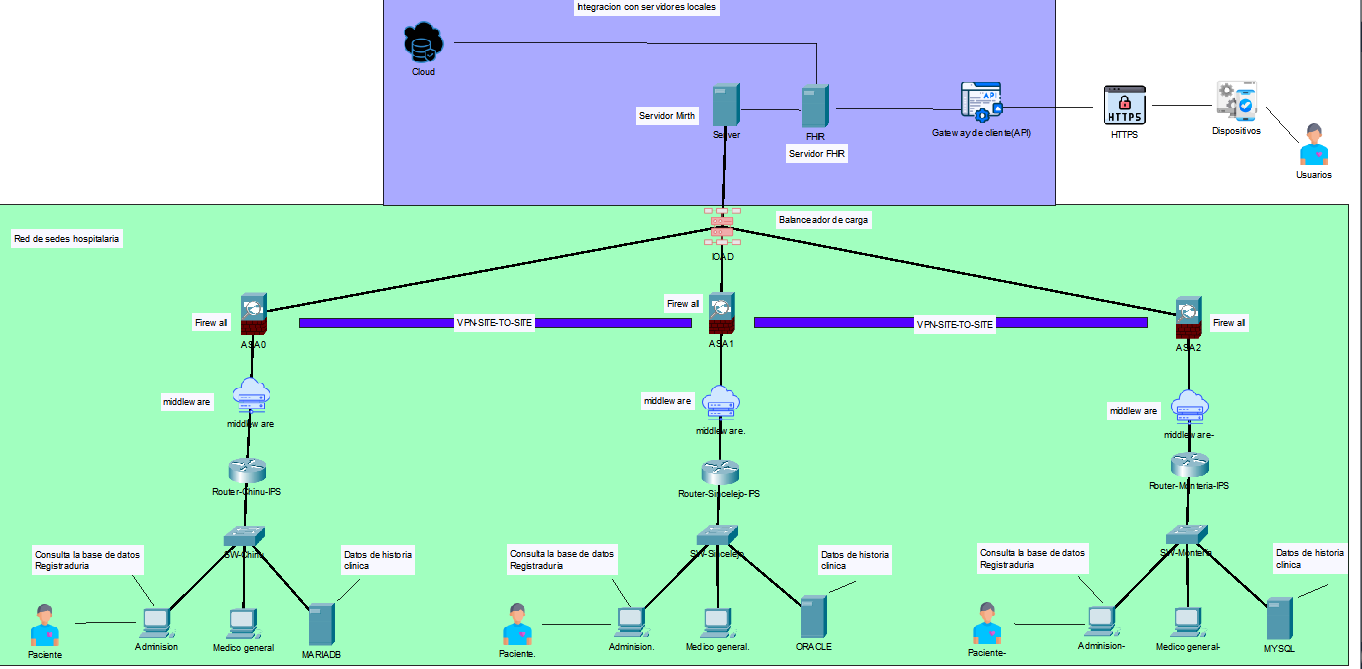
\includegraphics[width=\columnwidth]{fig_arquitectura.png}}

    \centering
    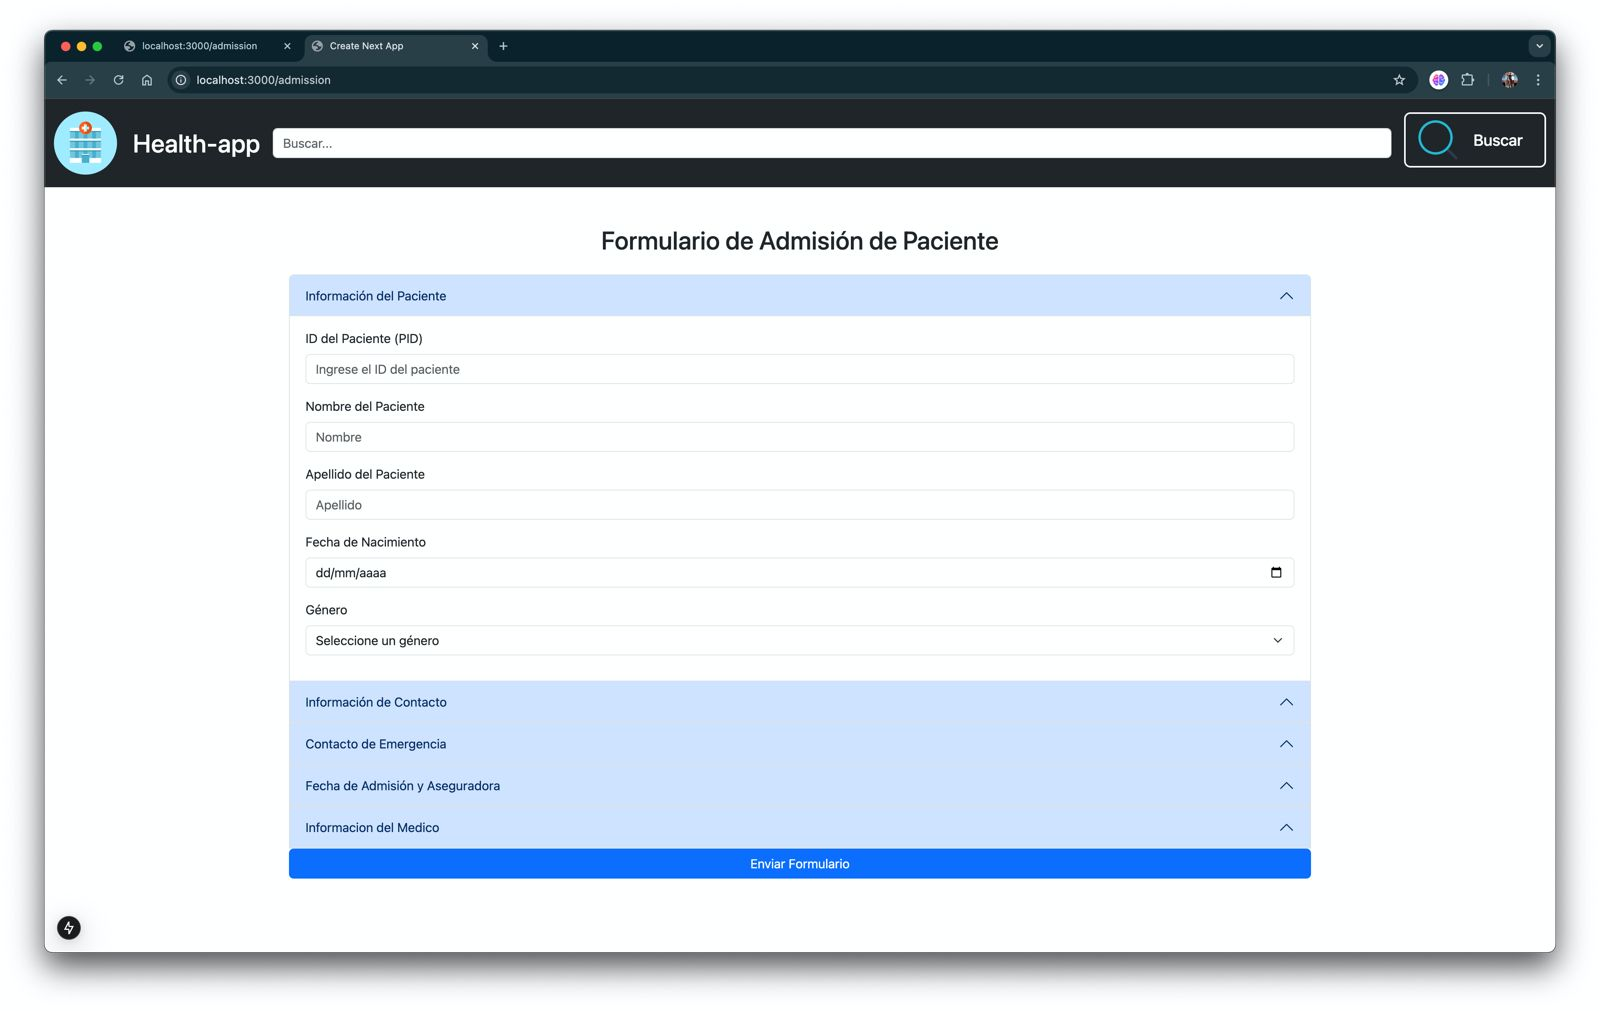
\includegraphics[width=0.5\linewidth]{fig_formulario.png}
    \caption{Enter Caption}
    \label{fig:placeholder}
\end{figure}
\begin{figure}
    \centering
    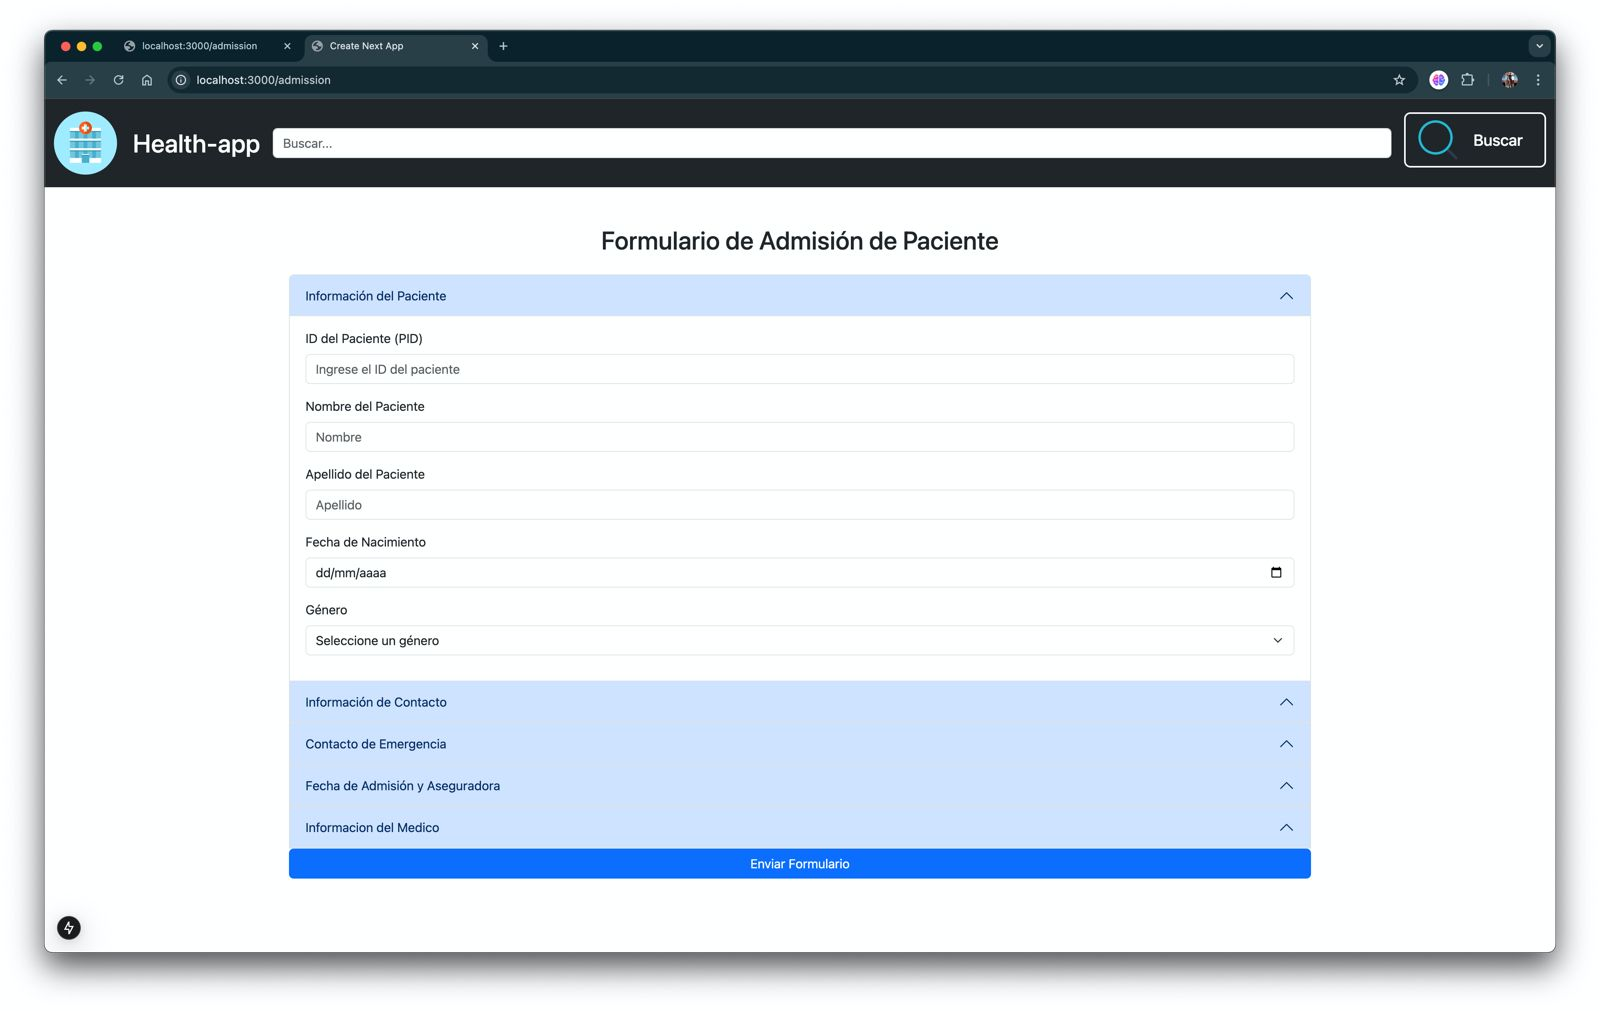
\includegraphics[width=0.5\linewidth]{fig_formulario.png}
    \caption{Enter Caption}
    \label{fig:placeholder}
\end{figure}
\caption{Arquitectura distribuida del prototipo. Nodos hospitalarios
independientes con HAPI FHIR y PostgreSQL, autenticaci\'on OAuth2
mediante Keycloak y monitoreo centralizado con Prometheus y Grafana.}
\label{fig:arq}
\end{figure}

La Tabla~\ref{tab:componentes} describe los componentes principales
del sistema, su rol en la arquitectura y la tecnolog\'ia de vanguardia
que representa cada uno.

\begin{table}[htbp]
\caption{Stack Tecnol\'ogico del Prototipo Distribuido FHIR}
\label{tab:componentes}
\begin{center}
\renewcommand{\arraystretch}{1.2}
\begin{tabular}{|p{1.9cm}|p{1.5cm}|p{3.9cm}|}
\hline
\textbf{Componente} & \textbf{Versi\'on} & \textbf{Rol en la arquitectura} \\
\hline
HAPI FHIR & 6.x (R4) & Servidor FHIR; expone API REST cl\'inica \\
\hline
Citus PostgreSQL & 12.x & Persistencia distribuida coordinator-worker \\
\hline
Docker Compose & 3.8 & Orquestaci\'on de contenedores y redes \\
\hline
React & 18.x & Frontend cl\'inico (admisi\'on, triage, reportes) \\
\hline
Keycloak & 22.x & Gesti\'on de identidad OAuth2/JWT/SMART on FHIR \\
\hline
Prometheus & 2.x & Scraping de m\'etricas de infraestructura \\
\hline
Grafana & 10.x & Visualizaci\'on de disponibilidad y rendimiento \\
\hline
\end{tabular}
\end{center}
\end{table}

\subsection{Fase 2 --- Despliegue de Infraestructura (Sprint 2)}

Se implement\'o la infraestructura mediante Docker Compose con redes
virtuales aisladas por nodo. Cada nodo hospitalario incluye: un
contenedor HAPI FHIR, un contenedor PostgreSQL, y configuraci\'on de
red interna. El nodo coordinador de Citus gestiona la distribuci\'on
horizontal de tablas cl\'inicas; los nodos worker almacenan los
\textit{shards} de datos. Keycloak fue configurado con un \textit{realm}
dedicado al sistema cl\'inico, definiendo roles de acceso por perfil
de usuario (m\'edico, enfermero, administrador). Prometheus realiza
\textit{scraping} de m\'etricas de cada contenedor cada 15 segundos;
Grafana expone \textit{dashboards} de disponibilidad, uso de CPU,
memoria y tiempos de respuesta.

\subsection{Fase 3 --- Desarrollo de Interfaz Cl\'inica (Sprint 3)}

Se desarroll\'o el frontend React con cuatro m\'odulos funcionales:
admisi\'on de pacientes, triage, historia cl\'inica y reportes. El
flujo operacional sigue cuatro pasos:

\textbf{Paso 1. Admisi\'on:} El usuario registra la informaci\'on
b\'asica del paciente desde el m\'odulo de admisi\'on (Fig.~\ref{fig:formulario}).

\textbf{Paso 2. Conversi\'on FHIR:} Los datos son transformados en
un recurso FHIR tipo \texttt{Patient} y enviados al servidor HAPI
FHIR del nodo activo.

\textbf{Paso 3. Persistencia distribuida:} HAPI FHIR almacena el
recurso en PostgreSQL gestionado por Citus~\cite{b6,b7}.

\textbf{Paso 4. Consulta cl\'inica:} Los m\'odulos de triage e historia
cl\'inica recuperan recursos mediante peticiones RESTful \texttt{GET}.

\begin{figure}[htbp]
\centerline{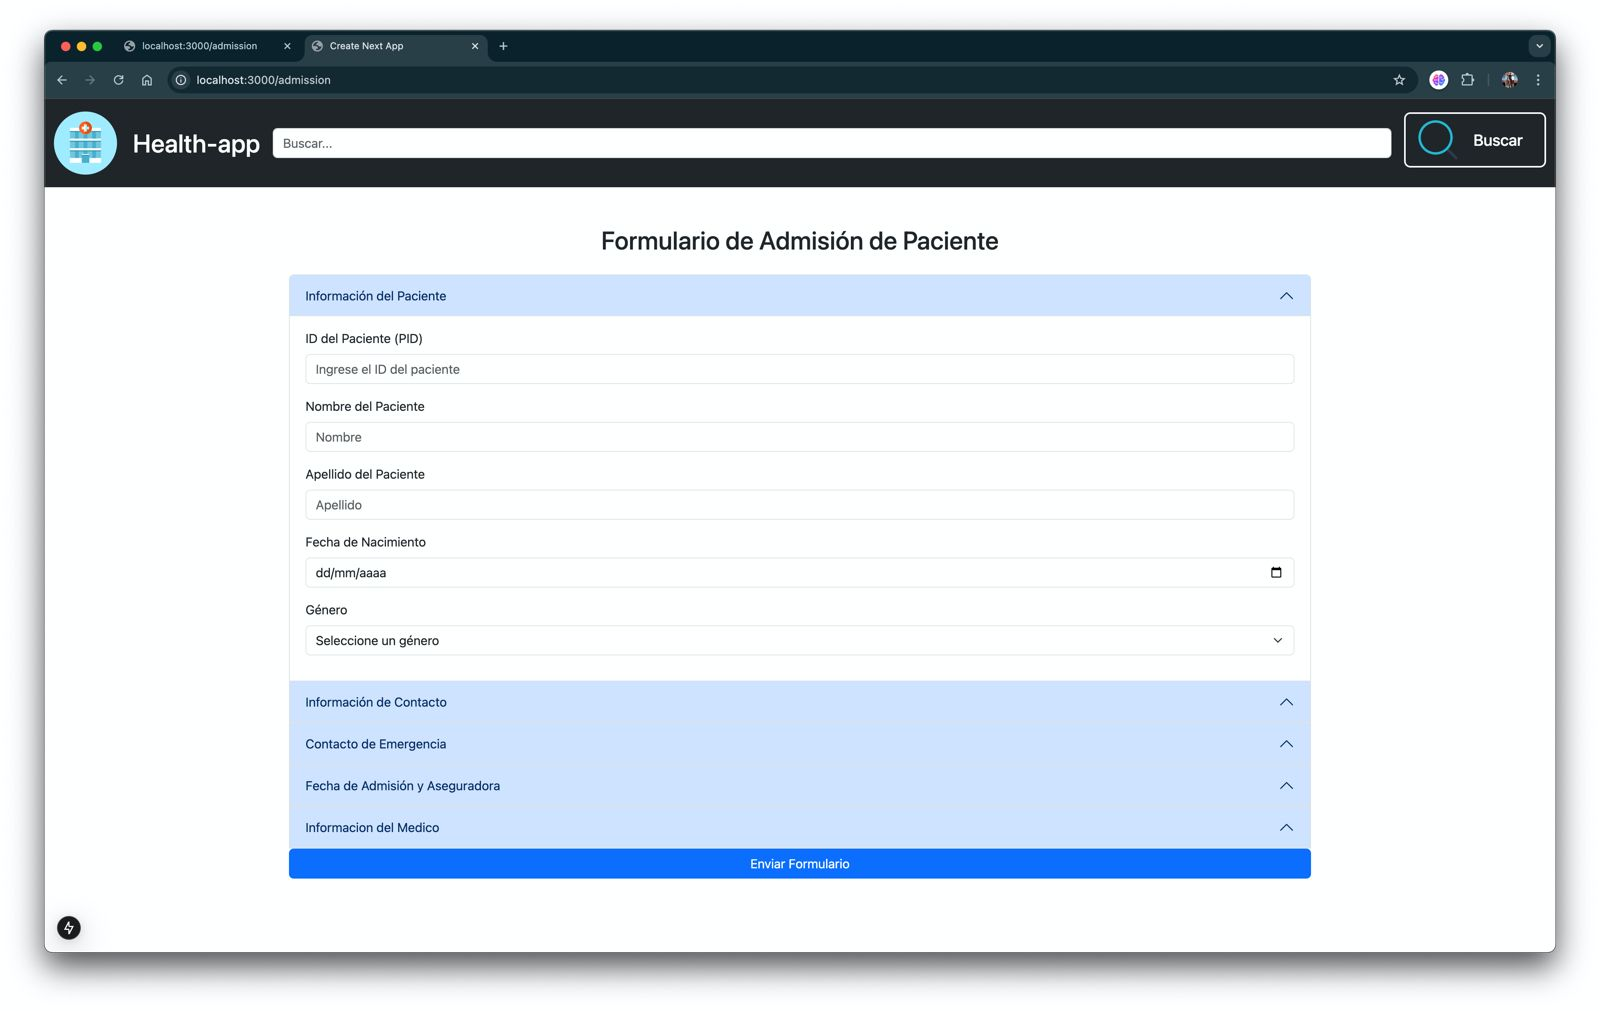
\includegraphics[width=\columnwidth]{fig_formulario.jpg}}
\caption{Formulario de admisi\'on del paciente. Captura tipo de documento,
nombre, fecha de nacimiento, sexo, g\'enero, discapacidad y municipio.
Fuente: prototipo historia cl\'inica distribuida FHIR (may-2026).}
\label{fig:formulario}
\end{figure}

La seguridad fue implementada con OAuth2 y tokens JWT mediante Keycloak
(Fig.~\ref{fig:login}): (1) el usuario inicia sesi\'on en Keycloak;
(2) Keycloak genera un token JWT firmado; (3) el frontend lo env\'ia
al servidor HAPI FHIR; (4) HAPI FHIR valida el token antes de procesar
la solicitud.

\begin{figure}[htbp]
\centerline{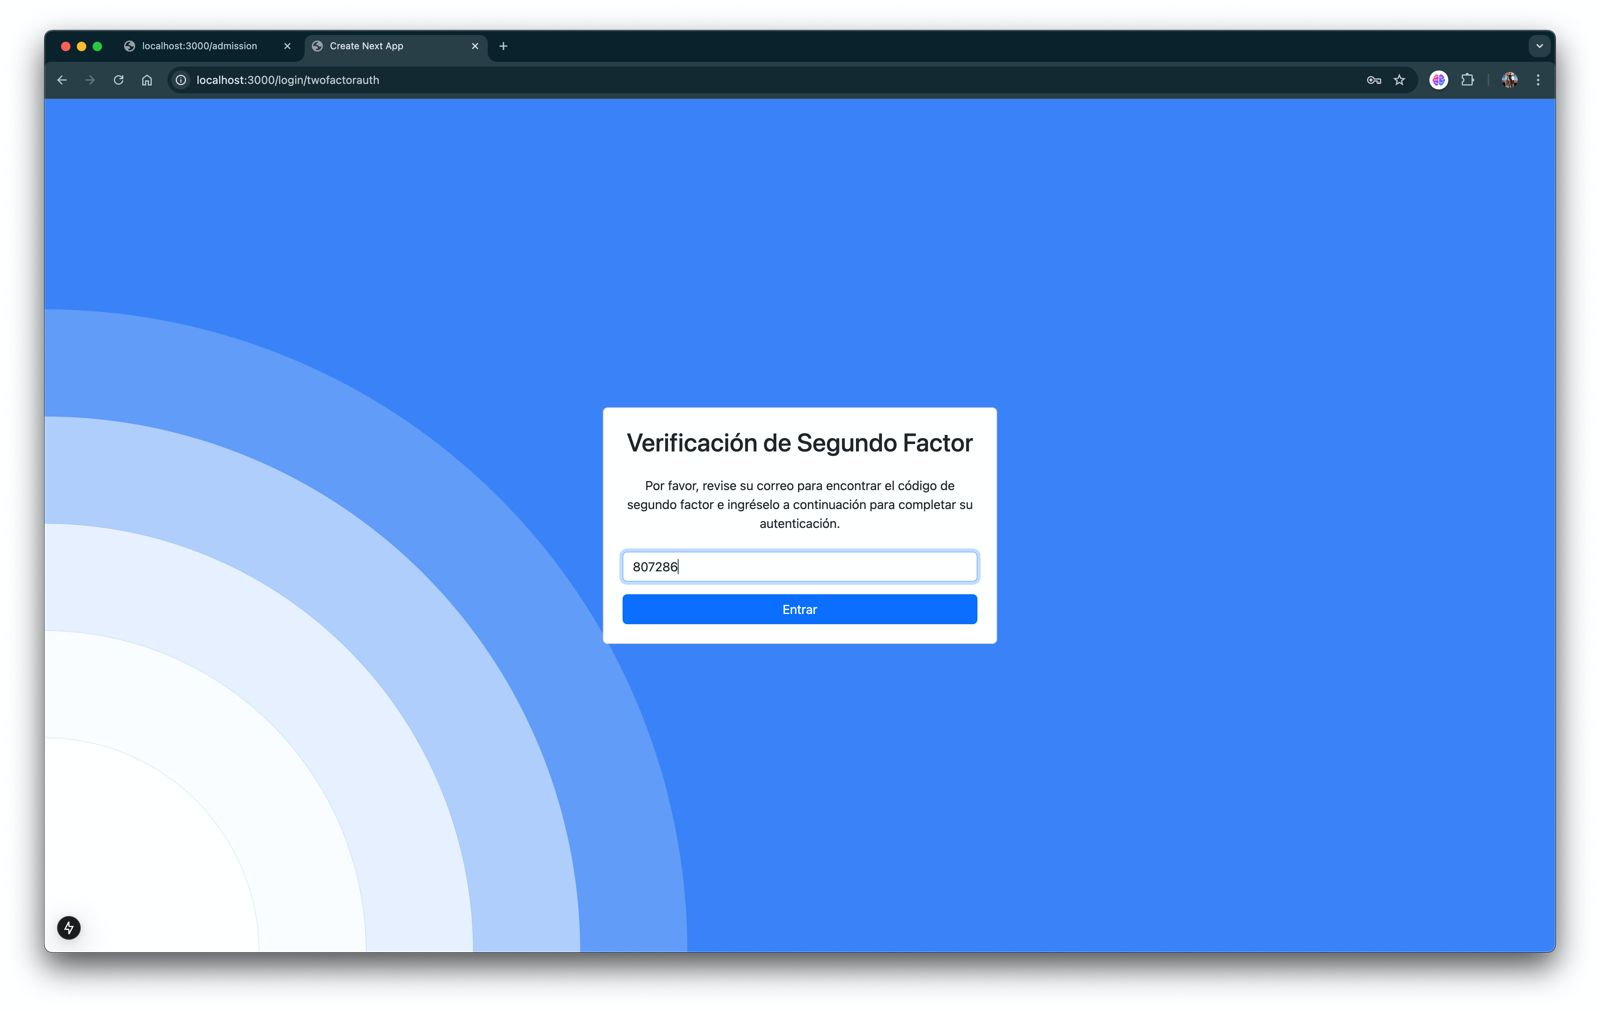
\includegraphics[width=0.7\columnwidth]{fig_login.jpg}}
\caption{Pantalla de autenticaci\'on OAuth2/JWT del sistema.
Keycloak gestiona la autorizaci\'on de acceso a los nodos FHIR.
Fuente: prototipo historia cl\'inica distribuida FHIR (may-2026).}
\label{fig:login}
\end{figure}

\subsection{Fase 4 --- Validaci\'on Funcional (Sprint 4)}

Se realizaron pruebas funcionales estructuradas como experimentos
por componente tecnol\'ogico, cuyos resultados se detallan en la
secci\'on~\ref{sec:resultados}. Las pruebas incluyeron: disponibilidad
de nodos, exposici\'on de recursos FHIR, flujo completo de admisi\'on
y consulta, autenticaci\'on OAuth2/JWT, y tolerancia a fallos mediante
desconexi\'on controlada de nodos.

% ============================================================
\section{Resultados y Experimentos}
\label{sec:resultados}

Los resultados se presentan organizados como experimentos por componente
tecnol\'ogico, siguiendo el stack definido en la Fase 1.

\subsection{Experimento 1 --- Disponibilidad de Nodos FHIR}

Se verific\'o la disponibilidad de cada nodo hospitalario mediante
consultas \texttt{GET /fhir/metadata} al \textit{capability statement}
de cada instancia HAPI FHIR. Los tres nodos respondieron con c\'odigo
HTTP 200 y el documento de capacidades FHIR R4 completo, confirmando
la operatividad del servidor. La Tabla~\ref{tab:disponibilidad} resume
los resultados.

\begin{table}[htbp]
\caption{Resultados de Disponibilidad de Nodos FHIR}
\label{tab:disponibilidad}
\begin{center}
\renewcommand{\arraystretch}{1.2}
\begin{tabular}{|p{1.6cm}|p{1.5cm}|p{1.2cm}|p{2.4cm}|}
\hline
\textbf{Nodo} & \textbf{Puerto} & \textbf{Estado} & \textbf{Recursos FHIR} \\
\hline
Nodo A & 8082 & Activo & Patient, Encounter \\
\hline
Nodo B & 8083 & Activo & Observation, Condition \\
\hline
Nodo C & 8084 & Activo & MedicationRequest \\
\hline
\end{tabular}
\end{center}
\end{table}

\subsection{Experimento 2 --- Recursos FHIR y Pipeline Cl\'inico}

Se valid\'o el ciclo completo de creaci\'on y consulta de recursos
cl\'inicos mediante peticiones REST. El Listado~\ref{lst:observation}
muestra la respuesta JSON del recurso \texttt{Observation} con c\'odigo
LOINC 8480-6 (presi\'on sist\'olica), confirmando la correcta
estructuraci\'on de los datos cl\'inicos conforme al est\'andar
FHIR R4~\cite{b1}.

\begin{lstlisting}[caption={Respuesta JSON del recurso FHIR Observation
(LOINC 8480-6 --- presi\'on sist\'olica). Evidencia de operatividad
del pipeline cl\'inico completo.},
label={lst:observation}]
{
  "resourceType": "Observation",
  "id": "obs-nodo-001",
  "status": "final",
  "code": {
    "coding": [{
      "system": "http://loinc.org",
      "code": "8480-6",
      "display": "Systolic blood pressure"
    }]
  },
  "subject": { "reference": "Patient/pat-001" },
  "valueQuantity": {
    "value": 120, "unit": "mmHg",
    "system": "http://unitsofmeasure.org"
  }
}
\end{lstlisting}

La Fig.~\ref{fig:obs} muestra la captura del endpoint en operaci\'on.

\begin{figure}[htbp]
\centerline{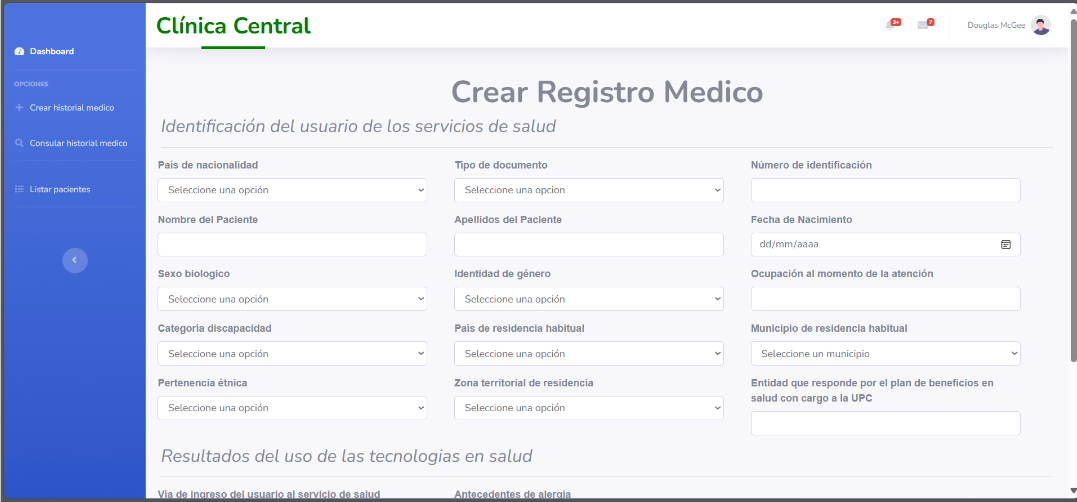
\includegraphics[width=\columnwidth]{fig_observation.jpg}}
\caption{Respuesta JSON del endpoint \texttt{/fhir/Observation}.
Recurso con c\'odigo LOINC 8480-6 en estado ``final'', con fuente y
versi\'on trazables. Fuente: prototipo historia cl\'inica distribuida FHIR (may-2026).}
\label{fig:obs}
\end{figure}

Se validaron todos los recursos cl\'inicos del prototipo:
\texttt{Patient}, \texttt{Encounter}, \texttt{Observation},
\texttt{Condition} y \texttt{MedicationRequest}, todos expuestos
mediante REST/JSON conforme a la especificaci\'on HL7 FHIR R4.

\subsection{Experimento 3 --- Persistencia Distribuida con Citus PostgreSQL}

La capa de persistencia utiliz\'o Citus PostgreSQL en topolog\'ia
coordinator-worker~\cite{b6,b7}. Las tablas de recursos FHIR fueron
distribuidas horizontalmente mediante la funci\'on
\texttt{create\_distributed\_table()}, permitiendo que los datos
cl\'inicos se almacenen y recuperen de forma transparente entre
m\'ultiples nodos de base de datos. Esta arquitectura de vanguardia
habilita escalado horizontal sin modificar la l\'ogica del servidor
HAPI FHIR, ya que Citus es completamente compatible con el protocolo
PostgreSQL est\'andar.

\subsection{Experimento 4 --- Autenticaci\'on OAuth2/JWT con Keycloak}

El flujo de autenticaci\'on fue validado end-to-end: el cliente React
obtiene un token JWT del servidor Keycloak, lo adjunta en la cabecera
\texttt{Authorization: Bearer} de cada petici\'on FHIR, y HAPI FHIR
verifica la firma del token antes de autorizar el acceso al recurso.
Keycloak 22.x implementa el est\'andar SMART on FHIR~\cite{bsmart},
proporcionando control de acceso basado en roles (RBAC) por tipo de
recurso cl\'inico.

\subsection{Experimento 5 --- Tolerancia a Fallos y Monitoreo}

Se realiz\'o desconexi\'on controlada de nodos Docker para evaluar la
continuidad operativa del sistema. Al desconectar un nodo, los
restantes continuaron respondiendo peticiones FHIR de forma
independiente, validando el patr\'on de aislamiento de fallos. El
monitoreo fue gestionado por Prometheus (m\'etricas de CPU, memoria,
latencia HTTP) y visualizado en Grafana con \textit{dashboards} en
tiempo real. La Tabla~\ref{tab:herramientas} resume el stack tecnol\'ogico
de vanguardia validado experimentalmente.

\begin{table}[htbp]
\caption{Herramientas de Vanguardia Validadas Experimentalmente}
\label{tab:herramientas}
\begin{center}
\renewcommand{\arraystretch}{1.2}
\begin{tabular}{|p{2.0cm}|p{1.7cm}|p{3.5cm}|}
\hline
\textbf{Herramienta} & \textbf{Protocolo} & \textbf{Resultado validado} \\
\hline
HAPI FHIR & REST/JSON & 5 tipos de recursos cl\'inicos operativos \\
\hline
Citus PostgreSQL & SQL & Persistencia distribuida coord.-worker \\
\hline
Docker Compose & Contenedores & Multi-nodo con aislamiento de fallos \\
\hline
React 18 & HTTP/JWT & Interfaz cl\'inica funcional 4 m\'odulos \\
\hline
Keycloak 22 & OAuth2/JWT & Autenticaci\'on SMART on FHIR validada \\
\hline
Prometheus & HTTP & Scraping de m\'etricas cada 15 s \\
\hline
Grafana & HTTP & Dashboards de disponibilidad en tiempo real \\
\hline
\end{tabular}
\end{center}
\end{table}

% ============================================================
\section{Discusi\'on}

Los cinco experimentos validan la viabilidad t\'ecnica de la
arquitectura propuesta. El uso de HL7 FHIR R4 garantiz\'o
compatibilidad con el est\'andar internacional, en l\'inea con lo
reportado por Gazzarata et al.~\cite{b3}, Vorisek et al.~\cite{b2}
y Lehne et al.~\cite{blehne}, quienes convergen en que FHIR es el
est\'andar dominante para la interoperabilidad cl\'inica digital.
La contenerizaci\'on con Docker simplific\'o el despliegue y el
aislamiento de nodos, facilitando las pruebas de tolerancia a fallos,
consistentemente con la propuesta de Mehta et al.~\cite{bmehta} sobre
arquitecturas FHIR con microservicios.

La integraci\'on de Keycloak con el perfil SMART on FHIR~\cite{bsmart}
representa un avance respecto al OAuth2 b\'asico documentado en la
literatura, al habilitar control de acceso granular por tipo de recurso
cl\'inico. La persistencia distribuida con Citus PostgreSQL~\cite{b6,b7}
permite escalar la capa de datos horizontalmente sin modificar la
l\'ogica FHIR, una ventaja arquitect\'onica no presente en los
prototipos monol\'iticos revisados en el estado del arte.

La principal limitaci\'on del prototipo es la ausencia de pruebas de
carga formales con m\'etricas cuantitativas de latencia, \textit{throughput}
y disponibilidad bajo concurrencia alta. El trabajo futuro debe
incorporar pruebas de rendimiento con JMeter o Locust, balanceo de
carga autom\'atico con NGINX o Traefik, y despliegue en infraestructura
cloud (Kubernetes en AWS o GCP) para validar el comportamiento en
condiciones de producci\'on.

% ============================================================
\section{Conclusiones}

Este trabajo demostr\'o que es posible construir un prototipo funcional
de historia cl\'inica electr\'onica distribuida e interoperable
utilizando exclusivamente tecnolog\'ias de vanguardia y c\'odigo
abierto: HL7 FHIR R4, HAPI FHIR, Docker Compose, Citus PostgreSQL,
Keycloak y Prometheus/Grafana. La metodolog\'ia Agile estructurada
en cuatro fases permiti\'o un desarrollo sistem\'atico con validaci\'on
experimental por componente.

Las contribuciones principales son: (1) una arquitectura de referencia
de nodos hospitalarios independientes e interoperables mediante HL7
FHIR R4; (2) una interfaz cl\'inica funcional para admisi\'on, triage
y consulta de recursos FHIR; (3) validaci\'on experimental de
comunicaci\'on REST/JSON, persistencia distribuida con Citus y
autenticaci\'on SMART on FHIR; y (4) un marco metodol\'ogico Agile
replicable para el desarrollo de infraestructuras cl\'inicas en
entornos acad\'emicos e institucionales latinoamericanos.

Como trabajo futuro se propone: incorporar pruebas de carga formales,
implementar balanceo de carga autom\'atico, despliegue en Kubernetes,
y extender la cobertura de recursos FHIR hacia perfiles IPS
(\textit{International Patient Summary}).

El repositorio del proyecto est\'a disponible en:
\url{https://github.com/jaiderreyes/historia-clinica-distribuida}

% ============================================================
\section*{Agradecimientos}

Los autores agradecen a la Corporaci\'on Universitaria Antonio Jos\'e
de Sucre (UAJS) por el apoyo institucional, y a los estudiantes
colaboradores del proyecto por su contribuci\'on al
desarrollo e implementaci\'on del sistema.

% ============================================================
\begin{thebibliography}{00}

\bibitem{b1}
HL7 International,
``FHIR Release 4 Specification,''
HL7 International, Ann Arbor, MI, 2019.
[En l\'inea]. Disponible en: \url{https://hl7.org/fhir/R4/}

\bibitem{b2}
C.~N. Vorisek et al.,
``Fast Healthcare Interoperability Resources (FHIR) for Interoperability
in Health Research: Systematic Review,''
\textit{JMIR Medical Informatics}, vol.~10, no.~7, p.~e35724, 2022.
DOI: \url{https://doi.org/10.2196/35724}

\bibitem{b3}
R. Gazzarata et al.,
``HL7 Fast Healthcare Interoperability Resources in digital healthcare
ecosystems: Scoping review,''
\textit{International Journal of Medical Informatics}, vol.~182,
p.~105318, 2024.
DOI: \url{https://doi.org/10.1016/j.ijmedinf.2023.105318}

\bibitem{b4}
G.~N. Bettoni et al.,
``Application of HL7 FHIR in a Microservice Architecture for Patient
Navigation on Registration and Appointments,''
\textit{arXiv preprint arXiv:2104.07661}, 2021.
[En l\'inea]. Disponible en: \url{https://arxiv.org/abs/2104.07661}

\bibitem{b5}
J. Mohammed and G. Hossain,
``Analyzing Healthcare Interoperability Vulnerabilities: Formal Modeling
and Graph-Theoretic Approach,''
\textit{arXiv preprint}, 2026.
[En l\'inea]. Disponible en: \url{https://arxiv.org}

\bibitem{b5_sec}
M. Pedrera-Jim\'enez et al.,
``Can OpenEHR, ISO 13606, and HL7 FHIR Work Together? An Agnostic
Approach for the Selection and Application of Electronic Health Record
Standards to the Next-Generation Health Data Spaces,''
\textit{Journal of Medical Internet Research}, vol.~25, p.~e51424, 2023.
DOI: \url{https://doi.org/10.2196/51424}

\bibitem{b6}
Citus Data,
``Citus: Distributed PostgreSQL — Concepts and Architecture,''
2024. [En l\'inea]. Disponible en: \url{https://docs.citusdata.com/}

\bibitem{b7}
Microsoft,
``Choosing a Distribution Column in Citus for PostgreSQL,''
2024. [En l\'inea]. Disponible en:
\url{https://learn.microsoft.com/en-us/azure/cosmos-db/postgresql/concepts-choose-distribution-column}

\bibitem{bwho}
World Health Organization,
``Patient Safety: Global Action on Patient Safety,''
WHO Press, Geneva, 2021.
[En l\'inea]. Disponible en: \url{https://www.who.int/news-room/fact-sheets/detail/patient-safety}

\bibitem{bbid}
Banco Interamericano de Desarrollo,
``Sistemas de Informaci\'on en Salud en Am\'erica Latina y el Caribe:
Diagn\'ostico y Hoja de Ruta,''
BID, Washington D.C., 2022.
[En l\'inea]. Disponible en: \url{https://publications.iadb.org}

\bibitem{bminsal}
Ministerio de Salud y Protecci\'on Social de Colombia,
``Marco de Interoperabilidad para el Sector Salud de Colombia,''
MinSalud, Bogot\'a, 2023.
[En l\'inea]. Disponible en: \url{https://www.minsalud.gov.co}

\bibitem{blehne}
M. Lehne et al.,
``The use of FHIR in digital health --- a review of the scientific
literature,''
\textit{Studies in Health Technology and Informatics}, vol.~267,
pp.~52--58, 2019.
DOI: \url{https://doi.org/10.3233/SHTI190813}

\bibitem{bsmart}
J.~C. Mandel et al.,
``SMART on FHIR: a standards-based, interoperable apps platform for
electronic health records,''
\textit{Journal of the American Medical Informatics Association},
vol.~23, no.~5, pp.~899--908, 2016.
DOI: \url{https://doi.org/10.1093/jamia/ocv189}

\bibitem{bmehta}
N. Mehta et al.,
``Deploying FHIR-Based Microservices with Docker and OAuth2 for Clinical
Data Exchange,''
\textit{Journal of Medical Internet Research}, vol.~24, no.~3,
p.~e30222, 2022.
DOI: \url{https://doi.org/10.2196/30222}

\bibitem{bdocker}
D. Merkel,
``Docker: Lightweight Linux Containers for Consistent Development and
Deployment,''
\textit{Linux Journal}, vol.~2014, no.~239, p.~2, 2014.

\bibitem{bkeycloak}
S. Trnkova and P. Mach,
``Keycloak as an Identity and Access Management Solution for Microservice
Architectures,''
in \textit{Proc. IEEE Int. Conf. on Software Architecture Companion
(ICSA-C)}, pp.~43--46, 2023.
DOI: \url{https://doi.org/10.1109/ICSA-C57050.2023.00017}

\bibitem{bprom}
B. Rabenstein and J. Volz,
``Prometheus: Up \& Running,''
O'Reilly Media, Sebastopol, CA, 2018.

\bibitem{bbigdata}
W. Raghupathi and V. Raghupathi,
``Big data analytics in healthcare: promise and potential,''
\textit{Health Information Science and Systems}, vol.~2, no.~1, p.~3,
2014.
DOI: \url{https://doi.org/10.1186/2047-2501-2-3}

\end{thebibliography}

\end{document}
